\subsection{Non-Verbal Learning Disabilities (NVLD)}
Non-verbal learning disabilities (NVLD) are neurodevelopmental conditions that impact a child's ability to understand and interpret non-verbal cues and information. Individuals with NVLD may struggle with social interactions, visual-spatial skills, motor coordination, and executive functioning. To develop interventions tailored to the needs of children with NVLD, it is essential to comprehend their unique user profile. This includes identifying their specific goals, psychographics, problems, characteristics and needs related to non-verbal learning.

\begin{figure}[H]
    \centering
    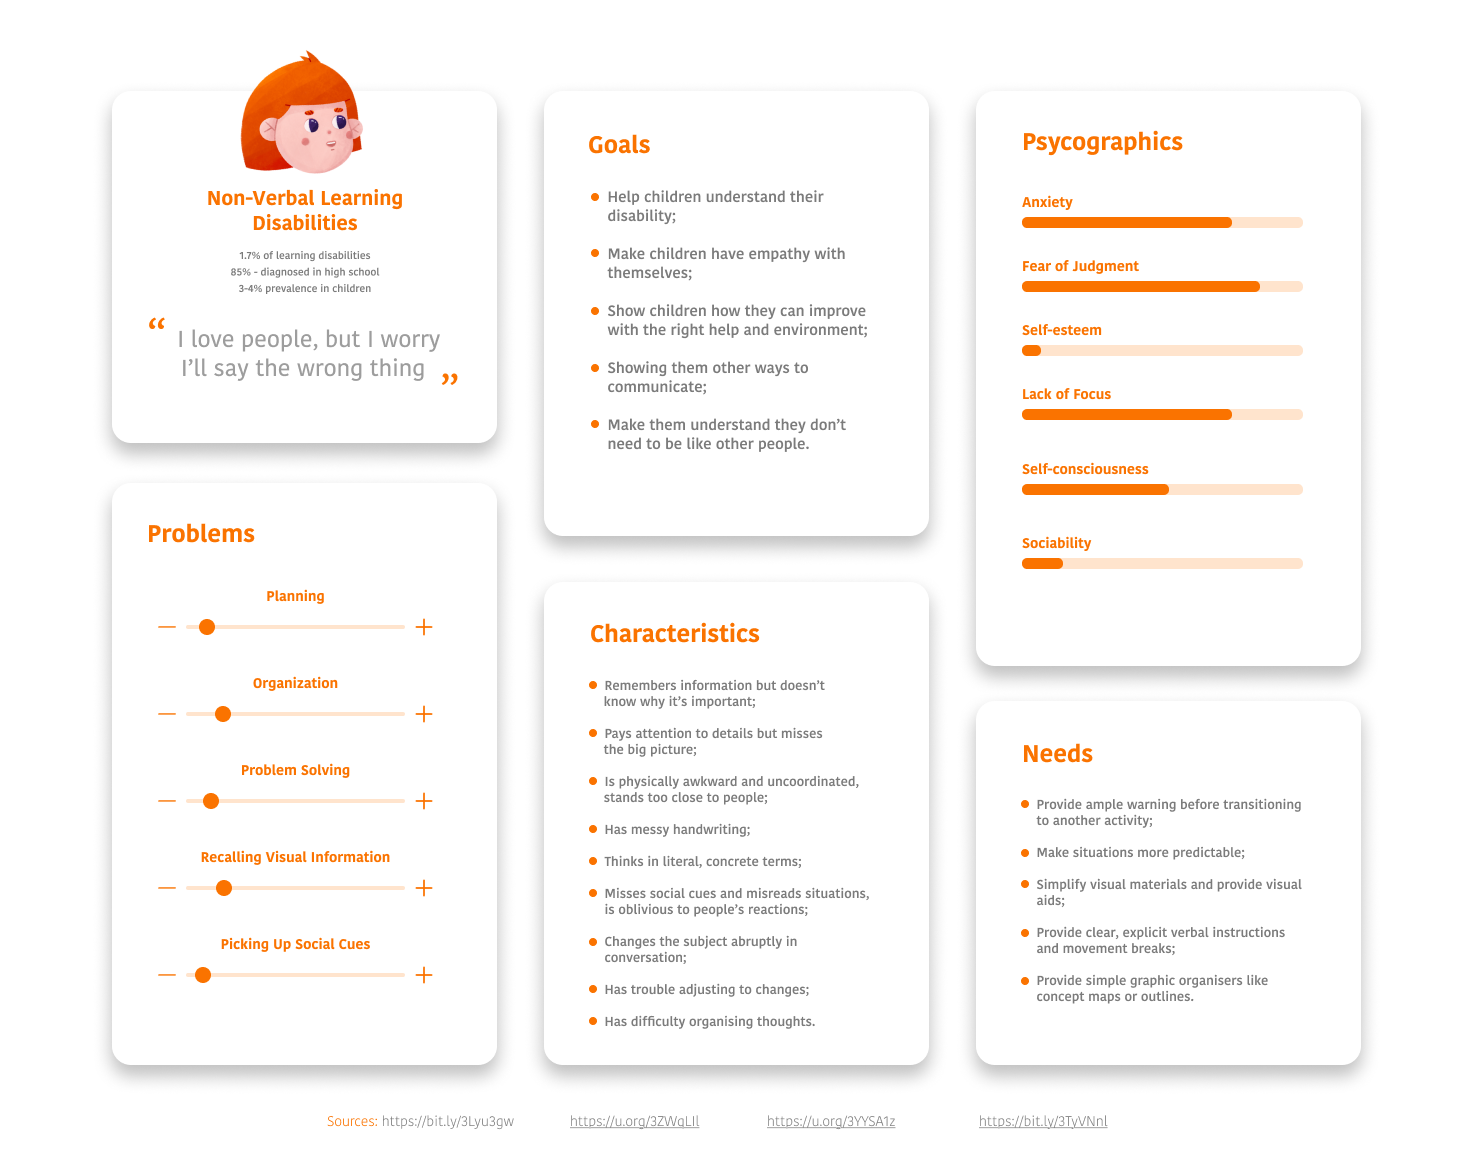
\includegraphics[width=0.8\linewidth]{Chapters/figma/Non-Verbal Learning Disabilities.png}
    \caption{Non-Verbal Learning Disabilities User Profile}
    \label{fig:nvldUserProfile}
\end{figure}

\paragraph{Goals}
\begin{itemize}
    \item \textbf{Help children understand their disability}: The mini-games aim to provide children with a comprehensive understanding of NVLD, its impact on their cognitive and social abilities, and how it shapes their unique strengths and challenges.
    \item \textbf{Foster empathy and self-acceptance}: By creating an environment of empathy and self-acceptance, the mini-games aim to help children develop a positive self-image, embrace their differences, and build resilience in the face of challenges.
    \item \textbf{Show children how they can improve}: The mini-games should demonstrate to children that with the right help, strategies, and supportive environment, they can improve their cognitive and social skills and navigate their daily lives more effectively.
    \item \textbf{Explore alternative communication methods}: The mini-games can introduce and explore different modes of communication to help children with NVLD find alternative ways to express themselves effectively.
    \item \textbf{Promote self-acceptance}: The mini-games aim to instill in children the understanding that they do not need to conform to societal expectations and that their unique strengths and perspectives are valuable.
\end{itemize}

\paragraph{Psycographics}
\begin{itemize}
    \item \textbf{High anxiety}: Children with NVLD often experience heightened levels of anxiety related to their difficulties in processing and understanding social and nonverbal cues \cite{understood_nvld_adult_2024}.
    \item \textbf{High fear of judgment}: Due to challenges in social interactions, children may have a heightened fear of being judged or evaluated negatively by others \cite{understood_nvld_adult_2024}.
    \item \textbf{Low self-esteem}: Struggles with cognitive and social skills can lead to lower self-esteem and self-worth \cite{understood_nvld_adult_2024}.
    \item \textbf{High lack of focus}: Difficulties in sustaining attention and focusing on relevant information may be characteristic of children with NVLD \cite{understood_nvld_2024}.
    \item \textbf{Average self-consciousness}: Children may have an average level of self-consciousness, as they are aware of their challenges but may not fully comprehend the underlying reasons \cite{understood_nvld_adult_2024}.
    \item \textbf{Low sociability}: Difficulties in social interactions may result in lower levels of social engagement and interaction \cite{understood_nvld_2024}.
\end{itemize}

\paragraph{Problems}
\begin{itemize}
    \item \textbf{Planning}: Difficulties in organizing and executing sequential tasks or activities effectively \cite{understood_nvld_adult_2024}.
    \item \textbf{Organization}: Challenges in managing and structuring information, materials, and personal belongings \cite{understood_nvld_adult_2024}.
    \item \textbf{Problem-solving}: Difficulties in identifying problems, generating solutions, and implementing strategies to resolve them effectively \cite{jama_nvld_2024}.
    \item \textbf{Recalling visual information}: Challenges in remembering and recalling visual information, such as faces, or visual details \cite{understood_nvld_2024}.
    \item \textbf{Picking up social cues}: Difficulty in understanding and interpreting nonverbal cues, gestures, facial expressions, and body language \cite{nationalLibraryMedicine}.
\end{itemize}

\paragraph{Characteristics}
\begin{itemize}
    \item \textbf{Remembering information without understanding its significance}: The ability to recall information but struggling to grasp its importance or connect it to broader contexts \cite{understood_nvld_2024}.
    \item \textbf{Attention to details at the expense of the big picture}: Focusing on specific details while overlooking the overall context or main idea \cite{understood_nvld_2024}.
    \item \textbf{Physical awkwardness and coordination difficulties}: Exhibiting motor coordination challenges, such as standing too close to others, clumsiness, or poor spatial awareness \cite{understood_nvld_2024}.
    \item \textbf{Messy handwriting}: Difficulty in producing legible and organized written work \cite{understood_nvld_2024}.
    \item \textbf{Literal, concrete thinking}: Tendency to think and interpret information in a literal and concrete manner, struggling with abstract or ambiguous concepts \cite{understood_nvld_2024}.
    \item \textbf{Missing social cues and misreading situations}: Difficulty in understanding and responding to social cues, resulting in misinterpretation of social situations and unawareness of others' reactions \cite{understood_nvld_2024}.
    \item \textbf{Abruptly changing the subject in conversation}: Shifting topics abruptly during conversations without recognizing the need for smooth transitions \cite{understood_nvld_2024}.
    \item \textbf{Difficulty adjusting to changes and transitions}: Resistance to changes in routines or environments, finding it challenging to adapt and adjust to new situations \cite{understood_nvld_2024}.
    \item \textbf{Difficulty organizing thoughts}: Struggles in structuring and organizing thoughts coherently, leading to difficulties in expressing ideas and communicating effectively \cite{understood_nvld_2024}.
\end{itemize}

\paragraph{Needs}
\begin{itemize}
    \item \textbf{Providing ample warning before transitioning}: Offering clear and advanced notice when transitioning from one activity or task to another, allowing children to mentally prepare and adjust \cite{understood_accommodations_2024}.
    \item \textbf{Making situations more predictable}: Creating predictable and structured environments to reduce anxiety and provide a sense of stability and security \cite{understood_accommodations_2024}.
    \item \textbf{Simplifying visual materials and providing visual aids}: Presenting visual materials in a simplified manner, using visual aids, diagrams, or illustrations to enhance understanding and facilitate information processing \cite{understood_accommodations_2024}.
    \item \textbf{Providing clear, explicit verbal instructions}: Offering precise and unambiguous verbal instructions to ensure clarity and comprehension, helping children to navigate through tasks and activities more effectively \cite{understood_accommodations_2024}.
    \item \textbf{Incorporating movement breaks}: Introducing regular movement breaks within the mini-games to allow children to release energy, improve focus, and enhance cognitive functioning \cite{understood_accommodations_2024}.
    \item \textbf{Providing simple graphic organizers}: Offering graphic organizers such as concept maps or outlines to assist children in organizing their thoughts, fostering structured thinking and facilitating effective communication \cite{understood_accommodations_2024}.
\end{itemize}
